\chapter{RF Amplifier}
\label{ch:rf_amplifier}
\raggedbottom

The RF amplifier provides gain to compensate for the insertion loss introduced by the Digital Step Attenuator (DSA). This gain helps prevent degradation of the overall noise figure (NF) of the receiver, thereby improving its sensitivity. However, the RF amplifier also limits the overall linearity of the receiver chain, so it is required to have high linearity. A good NF alone is not sufficient to achieve the main advantage of improved sensitivity, so the design requires a trade-off between linearity and noise performance.

\begin{figure}[H]
    \centering
    \vspace{-4pt}
    
\includegraphics[width=0.75\textwidth]{Amp_spc.png}
    \caption{Required RF amplifier specifications}
    \label{fig:rf_amp_specs}
\end{figure}

%=============================================================
\section{Proposed Topology}
\label{sec:proposed_topology}

The used topology utilises a differential cascode topology with active shunt-resistive feedback ($R_F$, $C_F$). The choice of a cascode configuration is driven by the strict requirements for high power handling and large output voltage swings. By distributing the voltage stress across stacked transistors, the maximum allowable $V_{DD}$ is safely increased, directly maximising the output voltage swing and significantly improving the 1-dB compression point ($P_\text{1dB}$). To achieve wideband input and output impedance matching, a resistive feedback network is integrated. This loop effectively lowers and stabilises the broadband input impedance, allowing for a well-behaved $50\,\Omega$ match ($S_{11}$) across an extended bandwidth while simultaneously flattening the forward transmission gain ($S_{21}$).

\begin{figure}[H]
    \centering
    \vspace{-4pt}
    
\includegraphics[width=0.65\textwidth]{rf_top.png}
    \caption{Proposed cascode topology with shunt-resistive feedback}
    \label{fig:proposed_topology}
\end{figure}

%=============================================================
\section{Design Challenges}
\label{sec:design_challenges}

\subsection{Choke Inductor for Wideband Operation}
\label{subsec:choke_inductor}

To maintain good matching across the wideband from 400\,MHz to 8\,GHz, the choke inductor must be sufficiently large at sub-1\,GHz frequencies to avoid leaking the RF signal into AC ground. Increasing the inductance value requires increasing the physical area, which reduces the self-resonance frequency and introduces higher losses that degrade the quality factor.

%-------------------------------------------------------------
\subsection{Trade-off Between Matching, Gain, NF, and Linearity}
\label{subsec:tradeoff_matching}

Decreasing the value of $R_F$ reduces the output and input impedance, improving impedance matching. It also introduces stronger negative feedback, which attenuates the effective voltage swing at the active gate, desensitising the circuit to device non-linearities and significantly boosting $P_\text{1dB}$ and IIP3. However, this degrades the gain due to the lower output impedance, and $R_F$ simultaneously injects higher thermal noise current $4kT/R_F$ directly into the input, causing the noise figure (NF) to rise. Optimising the value of the resistive feedback is therefore necessary to balance matching, gain, and NF simultaneously.

%-------------------------------------------------------------
\subsection{Cascode Gate Capacitor}
\label{subsec:cascode_cap}

Reducing the cascode gate capacitor increases the impedance seen from the source of the cascode device, which helps distribute the AC voltage swing between the main and cascode devices, preventing device breakdown. However, this reduction also decreases the output impedance and gain, increases the Miller effect which limits the wideband response, and upconverts the NF.

%-------------------------------------------------------------
\subsection{Trade-off Between Linearity and Gain}
\label{subsec:tradeoff_lin_gain}

Increasing the bias current raises the $g_m$ of the main device, which increases OIP3 but also increases gain. Since $\text{IIP3} = \text{OIP3} - G$, IIP3 remains approximately constant. To meet the required $\text{IIP3} = 30 - 12 = 18\,\text{dBm}$, simply increasing current is insufficient; the required OIP3 at the target gain cannot be achieved by current scaling alone.

%=============================================================
\section{Proposed Techniques to Increase Linearity}
\label{sec:linearity_techniques}

Since IIP3 is proportional to $g_m / g_{m3}$, where $g_{m3}$ is the third derivative of the drain current with respect to $V_{GS}$:
\begin{equation}
    \text{AIIP3} = \sqrt{\frac{4}{3} \frac{g_m}{g_{m3}}}, \qquad g_{m3} = \frac{1}{6} \frac{\partial^3 I_D}{\partial V_{GS}^3}
    \label{eq:IIP3}
\end{equation}

Boosting IIP3 can be achieved either by increasing $g_m$ or by reducing $g_{m3}$. Several techniques are discussed below.

%-------------------------------------------------------------
\subsection{Increasing $g_m$}
\label{subsec:increase_gm}

The main device is biased between $f_T$ and $NF_\text{min}$. Increasing $g_m$ can be achieved by increasing the current and the width to maintain the same optimal current density $J_\text{opt}$ for $f_T$ and $NF_\text{min}$. However, this also increases $g_{m3}$, though by a smaller ratio, allowing OIP3 to increase. The gain also increases, which prevents the required IIP3 from being met through this method alone.

%-------------------------------------------------------------
\subsection{Reducing $R_F$}
\label{subsec:reduce_RF}

Lowering the value of the shunt-feedback resistor introduces heavy negative feedback, which attenuates the input error voltage and significantly boosts the overall OIP3. However, this aggressively loads the output node, degrading both the gain and noise figure beyond acceptable specification limits.

%-------------------------------------------------------------
\subsection{Biasing at the $g_{m3}$ Zero-Crossing}
\label{subsec:gm3_zero}

Biasing a single main transistor directly at its intrinsic $g_{m3} = 0$ crossing point maximises linearity but introduces severe performance bottlenecks. Because this zero-crossing naturally occurs in the moderate inversion region, it degrades $NF_\text{min}$, yields a lower fundamental transconductance $g_m$, and reduces the cut-off frequency $f_T$ compared to strong inversion, directly degrading the forward gain $S_{21}$. Furthermore, because the $g_{m3}$ curve exhibits an exceptionally steep slope as it transitions through zero, the null point is highly unstable. Minor shifts due to process corners, voltage fluctuations, and temperature (PVT) variations easily displace the biasing away from the zero-crossing, causing large fluctuations in the actual $g_{m3}$ value and a severe drop in IIP3 that ultimately fails the linearity specifications.

\begin{figure}[H]
    \centering
    \vspace{-4pt}
    
\includegraphics[width=0.6\textwidth]{gm3_vgs.png}
    \caption{$g_{m3}$ curve vs.\ $V_{GS}$}
    \label{fig:gm3_curve}
\end{figure}

%-------------------------------------------------------------
\subsection{linearization Techniques}
\label{subsec:linearization}

\subsubsection{Feedforward linearization Technique}
\label{subsubsec:feedforward}

The feedforward technique improves linearity without sacrificing core stage gain by splitting the input RF signal into two parallel paths: a main non-linear amplification path and an auxiliary error-extraction path. The distortion products generated by the main amplifier are isolated in the error loop, amplified, and then recombined at the output with a 180° phase shift to cancel the third-order intermodulation (IMD3) products.

The primary drawback is NF degradation: the passive power splitters and delay elements required at the input port introduce insertion loss \textit{before} the first amplification stage. This loss attenuates the incoming signal and translates directly into a dB-for-dB increase in the overall noise figure, making it exceptionally difficult to meet stringent low-noise specifications. It also affects the S-parameters, including gain and input/output matching.

\begin{figure}[H]
    \centering
    \vspace{-4pt}
    
\includegraphics[width=0.7\textwidth]{feedforward.png}
    \caption{Feedforward linearization technique}
    \label{fig:feedforward}
\end{figure}

%-------------------------------------------------------------
\subsubsection{Derivative Superposition (Multi-Gate Biasing)}
\label{subsubsec:DS_technique}

The Derivative Superposition (DS) technique improves linearity by achieving third-order transconductance $g_{m3}$ cancellation through the parallel combination of a main and an auxiliary transistor~\cite{article}. Because the $g_{m3}$ characteristic transitions from a positive peak in the subthreshold (weak inversion) region to a negative peak in the moderate-to-strong inversion region, the two devices are biased differently to exploit this phase inversion. The primary transistor is biased in strong inversion to optimise high fundamental transconductance $g_m$, $f_T$, and $NF_\text{min}$, giving it a negative $g_{m3}$. Conversely, the auxiliary transistor is sized and intentionally biased in the subthreshold region where its $g_{m3}$ is positive. Tying the gates and drains of both devices together creates a composite third-order transconductance:
\begin{equation}
    g_{m3,\text{total}} = g_{m3,\text{main}} + g_{m3,\text{aux}} \approx 0
    \label{eq:gm3_total}
\end{equation}
that approaches zero over a wider $V_{GS}$ voltage swing, significantly boosting the composite IIP3. Because the auxiliary device operates in subthreshold, its DC current consumption is negligible, preventing significant power overhead or NF degradation. However, the primary drawback of this technique is that it only improves small-signal linearity; under large-signal excitation, the large input voltage swing drives the transistors out of their optimal bias points, causing the $g_{m3}$ cancellation to degrade rapidly.

\begin{figure}[H]
    \centering
    \vspace{-4pt}
    
\includegraphics[width=0.55\textwidth]{a-Derivative-superposition-b-Third-order-transconductance.png}
    \caption{Derivative Superposition (DS) technique}
    \label{fig:DS_technique}
\end{figure}

%=============================================================
\section{Design of Derivative Superposition linearization}
\label{sec:DS_design}

The Derivative Superposition (DS) technique represents the optimal choice for this wideband receiver architecture because it decouples input linearity from primary noise-matching and biasing constraints. Unlike alternative topologies that introduce lossy passive components or power-hungry auxiliary paths, DS achieves $g_{m3}$ cancellation without altering the optimum noise current density $J_\text{opt}$ of the core stage. This preserves the minimum noise figure $NF_\text{min}$ of the main amplifier, allowing the circuit to satisfy stringent IIP3 specifications while maintaining a low noise profile. Furthermore, because the cancellation relies on the combined, overlapping profiles of two parallel devices rather than a single highly sensitive zero-crossing point, the composite $g_{m3}$ null exhibits superior robustness against process corners and temperature variations, ensuring stable linearity yield across PVT.

\begin{figure}[H]
    \centering
    \vspace{-4pt}
    
\includegraphics[width=0.55\textwidth]{ds.png}
    \caption{DS technique schematic}
    \label{fig:DS_schematic}
\end{figure}

From a Taylor series expansion, the drain current can be expressed as:
\begin{equation}
    i_{DS} = g_m v_{gs} + g_{m2} v_{gs}^2 + g_{m3} v_{gs}^3 + \cdots
    \label{eq:taylor}
\end{equation}

The technique works by cancelling the $g_{m3}$ contributions of the two parallel devices, which have opposite signs, by summing their drain currents.

%-------------------------------------------------------------
\subsection{Derivative Superposition Testbench}
\label{subsec:DS_testbench}

The main device is placed with its biasing and sizing to preserve the required S-parameters.

\begin{figure}[H]
    \centering
    \vspace{-4pt}
    
\includegraphics[width=0.65\textwidth]{gm3_tb.png}
    \caption{DS testbench}
    \label{fig:DS_testbench}
\end{figure}

%-------------------------------------------------------------
\subsection{Width Sizing of the Auxiliary Transistor}
\label{subsec:aux_width}

The $g_{m3}$ curve of the auxiliary transistor scales with its width. The width is optimised to cancel the $g_{m3}$ of the main device, as shown in Figure~\ref{fig:gm3_sizing}.

\begin{figure}[H]
    \centering
    \vspace{-4pt}
    
\includegraphics[width=0.65\textwidth]{gm3_Withsizingaux.png}
    \caption{Total $g_{m3}$ with auxiliary transistor sizing}
    \label{fig:gm3_sizing}
\end{figure}

%-------------------------------------------------------------
\subsection{Biasing of the Auxiliary Transistor}
\label{subsec:aux_bias}

Changing the shift voltage from $V_{GS}$ shifts the $g_{m3}$ curve of the auxiliary device, which in turn shifts the biasing point. The shift voltage is selected such that the total $g_{m3}$ equals zero at the required $V_{GS}$ of the main device.

\begin{figure}[H]
    \centering
    \vspace{-4pt}
    
\includegraphics[width=0.8\textwidth]{gm3_vsh.png}
    \caption{$g_{m3}$ of the auxiliary device vs.\ shift voltage}
    \label{fig:gm3_shift}
\end{figure}

\begin{figure}[H]
    \centering
    \vspace{-4pt}
    
\includegraphics[width=0.8\textwidth]{gm3t_vsh.png}
    \caption{Total $g_{m3}$ for different shift voltages}
    \label{fig:gm3_total_shift}
\end{figure}

%-------------------------------------------------------------
\subsection{OIP3 at Band Edges vs.\ Auxiliary Gate Capacitor}
\label{subsec:OIP3_Caux}

This behaviour highlights a fundamental limitation of the conventional DS technique. At DC and low frequencies, $g_{m3}$ cancellation works well with a small auxiliary capacitance $C_\text{aux}$, because the transistor operates as a memoryless small-signal device. Increasing $C_\text{aux}$ under these conditions introduces an unnecessary high-frequency phase shift that distorts the ideal low-frequency vector cancellation of $g_{m3}$, causing the 400\,MHz linearity to degrade. Conversely, at high frequencies (8\,GHz), finite internal parasitic capacitances and second-harmonic feedback loops introduce severe phase shifts that lead to vector misalignment in the cancellation mechanism. A higher $C_\text{aux}$ provides the necessary phase alignment and low AC impedance to compensate for these parasitics, restoring robust vector cancellation at the high-frequency band edge. Therefore, a carefully optimised intermediate capacitance value must be selected to balance low-frequency memoryless cancellation with high-frequency phase matching.

\begin{figure}[H]
    \centering
    \vspace{-4pt}
    
\includegraphics[width=0.6\textwidth]{caux.png}
    \caption{Auxiliary gate capacitor $C_\text{aux}$}
    \label{fig:Caux}
\end{figure}

\begin{figure}[H]
    \centering
    \vspace{-4pt}
    
\includegraphics[width=0.65\textwidth]{OIP3_CAUX.png}
    \caption{OIP3 at band edges vs.\ $C_\text{aux}$}
    \label{fig:OIP3_vs_Caux}
\end{figure}

%=============================================================
\section{RF Theory of Derivative Superposition}
\label{sec:DS_theory}

In a weakly non-linear, un-degenerated ($L = 0$) stage with neglected $C_{gd}$, third-order intermodulation products stem entirely from the native $g_3 v_{gs}^3$ term. However, adding a source inductor $L$ creates a feedback loop that feeds second-harmonic drain currents ($2\omega_a$, $2\omega_b$) generated by $g_2 v_{gs}^2$ back into the gate-source voltage $v_{gs}$. These $2\omega$ components mix again with the fundamental tones within the $g_2$ non-linearity, generating secondary IMD3 responses at $2\omega_a \pm \omega_b$ and $2\omega_b \pm \omega_a$. Thus, second-order non-linearities directly degrade third-order linearity at high frequencies.

\begin{figure}[H]
    \centering
    \vspace{-4pt}
    
\includegraphics[width=0.65\textwidth]{NONLINEAR.png}
    \caption{Small-signal non-linear model of FET}
    \label{fig:FET_model}
\end{figure}

Even when source degeneration is eliminated ($L = 0$), the intrinsic parasitic capacitances of the transistor ($C_{gd}$ and $C_{gs}$) establish an alternative high-frequency feedback path that triggers the same second-order interaction loop. At high frequencies, the low impedance of the gate-drain capacitance ($1/j\omega C_{gd}$) allows second-harmonic drain currents ($2\omega_a$, $2\omega_b$) generated by $g_2$ to leak back to the input gate node. This fed-back voltage drops across the capacitive divider formed by $C_{gd}$ and $C_{gs}$, modulating the internal gate-source voltage $v_{gs}$ with a second-harmonic component. This $2\omega$ voltage then mixes again with the fundamental tones within the $g_2$ non-linearity, producing secondary IMD3 responses ($2\omega_a \pm \omega_b$ and $2\omega_b \pm \omega_a$). Consequently, high-frequency IMD3 degradation occurs even without source inductors.

%=============================================================
\section{Modified Superposition Technique}
\label{sec:modified_DS}

This modified technique inserts a phase difference between the main path and the auxiliary path to achieve phase alignment between the third-order component of the auxiliary device and the combined third- and second-order components of the main device. This can be visualised as a vector cancellation problem, as shown in Figure~\ref{fig:phase_alignment}.

\begin{figure}[H]
    \centering
    \vspace{-4pt}
    
\includegraphics[width=0.4\textwidth]{PHASOR.png}
    \caption{Phase alignment of IM3 vectors}
    \label{fig:phase_alignment}
\end{figure}

\begin{figure}[H]
    \centering
    \vspace{-4pt}
    
\includegraphics[width=0.65\textwidth]{MODF.png}
    \caption{Modified superposition technique}
    \label{fig:modified_DS}
\end{figure}

However, this technique requires the use of a degeneration inductor, which degrades the NF and causes gain to decrease across the wideband, limiting the wideband frequency response.

%=============================================================
\section{Proposed Modification to the Superposition Technique}
\label{sec:proposed_modification}

As an alternative to conventional modified DS architectures, this work proposes a novel modification that places a dedicated phase-shifting inductor ($L_G$) directly at the gate of the auxiliary transistor. Traditional architectures often utilise split source-degeneration inductors to generate the required high-frequency phase shift~\cite{1320540}; however, this severely compromises overall performance by introducing negative feedback that degrades the fundamental transconductance ($g_m$), lowers the power gain ($S_{21}$), and corrupts the noise figure (NF). In contrast, placing the tuning inductor exclusively in the input path of the auxiliary device isolates the primary amplification stage from destructive fundamental feedback. The auxiliary gate inductor forms a local passive $LC$ network with the device's intrinsic gate-source capacitance ($C_{gs,\text{aux}}$), introducing a precise, frequency-dependent phase lag to the fundamental signal before it drives the auxiliary path. This rotates the auxiliary path's IMD3 vector to achieve perfect destructive interference with the main path's distortion at the 8\,GHz band edge. Because the main amplifier's source remains directly grounded (or uncompromised), this architecture yields optimal high-frequency vector cancellation while maintaining maximum fundamental gain, preserving a low noise figure, and minimising interaction with the primary input matching network ($S_{11}$).

\begin{figure}[H]
    \centering
    \vspace{-4pt}
    
\includegraphics[width=0.4\textwidth]{LCOMP.png}
    \caption{Proposed modified Derivative Superposition with auxiliary gate inductor}
    \label{fig:proposed_modified_DS}
\end{figure}

%-------------------------------------------------------------
\subsection{Phase Difference Between IM3 Drain Currents With and Without Compensation}
\label{subsec:phase_diff}

To evaluate the high-frequency vector cancellation of the DS technique, the relative phase difference ($\Delta\theta = \angle i_{DS3,a} - \angle i_{DS3,b}$) between the third-order intermodulation drain currents of the main ($M_a$) and auxiliary ($M_b$) transistors was simulated up to 9\,GHz. At low frequencies below 1\,GHz, the compensation inductor introduces no variance. The critical performance divergence occurs above 4\,GHz. Without compensation ($L_\text{comp} = 1\,\text{pH}$), the phase difference drops continuously to 175.5° at 9\,GHz, degrading the anti-phase cancellation condition. Conversely, the optimised inductor ($L_\text{comp} = 400\,\text{pH}$) introduces a targeted inductive delay that effectively counters the capacitive phase rotation of the auxiliary gate path. This stabilises the high-frequency phase trajectory, forcing the phase difference to cross precisely through the ideal 180° anti-phase target at 9\,GHz and preserving wideband linearity across the upper band edge.

\begin{figure}[H]
    \centering
    \vspace{-4pt}
    
\includegraphics[width=0.65\textwidth]{phase_diff.png}
    \caption{Phase difference between third-order harmonic drain currents with and without $L_\text{comp}$}
    \label{fig:phase_diff}
\end{figure}

%-------------------------------------------------------------
\subsection{Total IM3 Drain Currents With and Without Compensation}
\label{subsec:IM3_total}

The improved phase alignment results in better cancellation of the third-order harmonic current above 4\,GHz.

\begin{figure}[H]
    \centering
    \vspace{-4pt}
    
\includegraphics[width=0.65\textwidth]{id3t.png}
    \caption{Total third-order harmonic drain current with and without compensation}
    \label{fig:IM3_total}
\end{figure}

%=============================================================
\section{OIP3 at Band Edges After the Proposed Gate Inductor}
\label{sec:OIP3_Lcomp}

The simulation results across the operating band demonstrate that the proposed gate inductor has no significant impact on low-frequency linearity, while profoundly enhancing high-frequency performance.

\begin{figure}[H]
    \centering
    \vspace{-4pt}
    
\includegraphics[width=0.65\textwidth]{oip3_lcomp.png}
    \caption{OIP3 improvement with $L_\text{comp}$}
    \label{fig:OIP3_Lcomp}
\end{figure}

%-------------------------------------------------------------
\subsection{NF With and Without the Proposed Gate Inductor}
\label{subsec:NF_Lcomp}

The proposed gate inductor introduces no significant degradation to the total NF.

\begin{figure}[H]
    \centering
    \vspace{-4pt}
    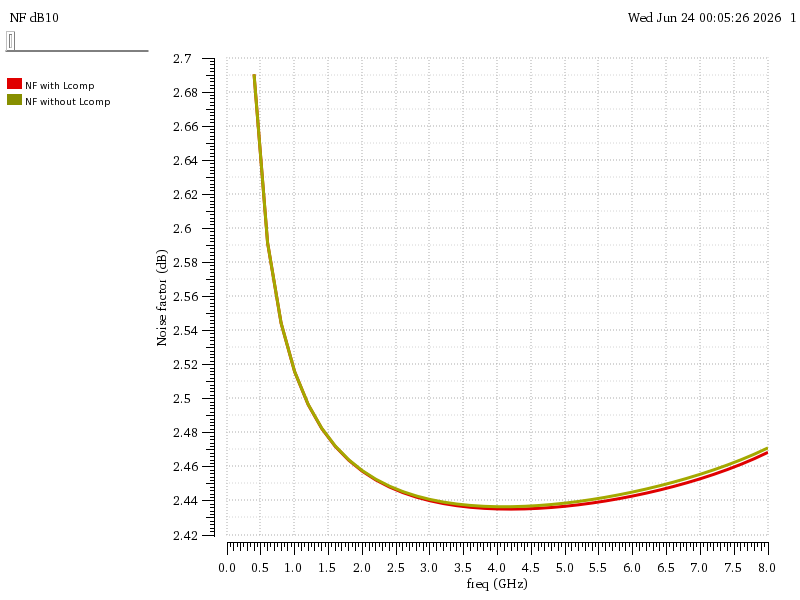
\includegraphics[width=0.65\textwidth]{chapter5_Yassin/images/NF_Lcomp.png}
    \caption{NF with and without $L_\text{comp}$}
    \label{fig:NF_Lcomp}
\end{figure}

%=============================================================
\section{Comparison of OIP3 Across Frequency}
\label{sec:OIP3_comparison}

The proposed gate-inductor modification ($L_\text{comp}$) maintains a remarkably flat and elevated linearity profile across the entire band. Below 1.5\,GHz, the proposed and conventional DS curves track identically, confirming that the inductor introduces no performance penalties under quasi-static conditions. At higher frequencies, the passive $LC$ network formed by $L_\text{comp}$ and the auxiliary gate-source capacitance introduces the necessary fundamental phase lag to realign the distortion vectors. At the critical 8\,GHz band edge, the proposed topology achieves an $\text{OIP}_3$ of 30.6\,dBm, providing a 2\,dB improvement over conventional DS and a 4.6\,dB boost over the baseline receiver without linearization. This robustly validates the capability of the proposed technique to sustain precise distortion cancellation across the full wideband spectrum.

\begin{figure}[H]
    \centering
    \vspace{-4pt}
    
\includegraphics[width=0.75\textwidth]{oip3_with_lin.png}
    \caption{OIP3 vs.\ frequency: no linearization, conventional DS, and proposed modified DS}
    \label{fig:OIP3_comparison}
\end{figure}

%=============================================================
\section{S-Parameters With and Without linearization}
\label{sec:S_params_DS}

As expected, the Derivative Superposition technique does not significantly affect the S-parameters, since the auxiliary device operates in the subthreshold region and carries negligible DC current.

%-------------------------------------------------------------
\subsection{Return Loss With and Without Derivative Superposition}
\label{subsec:RL_DS}

The auxiliary device adds a parallel input impedance with the main device, which reduces the overall input impedance and improves input matching ($S_{11}$). The output matching ($S_{22}$) is not affected.

\begin{figure}[H]
    \centering
    \vspace{-4pt}
    
\includegraphics[width=0.75\textwidth]{s11_withlin.png}
    \caption{$S_{11}$ with and without Derivative Superposition}
    \label{fig:S11_DS}
\end{figure}

%-------------------------------------------------------------
\subsection{Gain With and Without Derivative Superposition}
\label{subsec:gain_DS}

The gain shows a small increase due to the slight increase in overall current and total $g_m$ contributed by the auxiliary device.

\begin{figure}[H]
    \centering
    \vspace{-4pt}
    
\includegraphics[width=0.75\textwidth]{s21_withlin.png}
    \caption{$S_{21}$ with and without Derivative Superposition}
    \label{fig:S21_DS}
\end{figure}

%-------------------------------------------------------------
\subsection{Noise Figure With and Without Derivative Superposition}
\label{subsec:NF_DS}

The overall NF is slightly reduced, consistent with the small gain increase, since the auxiliary device contributes minimal additional noise due to its small DC current.

\begin{figure}[H]
    \centering
    \vspace{-4pt}
    
\includegraphics[width=0.75\textwidth]{nf_withlin.png}
    \caption{NF with and without Derivative Superposition}
    \label{fig:NF_DS}
\end{figure}

%=============================================================
\section{Design of the Choke Inductor}
\label{sec:choke_design}

\subsection{Spiral Inductor}
\label{subsec:spiral_inductor}

Conventional on-chip planar spiral inductors are highly constrained when realising the large inductance values required for wideband RF choke applications. Attempting to increase the inductance by adding more turns. This expanded area increases the parasitic capacitance. Consequently, the self-resonance frequency ($f_\text{SRF}$) drops much, with degraded Quality factor 

\begin{figure}[H]
    \centering
    \vspace{-4pt}
    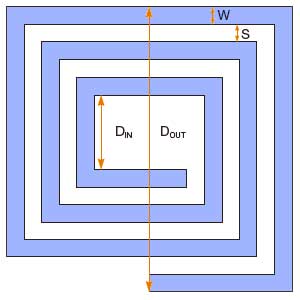
\includegraphics[width=0.4\textwidth]{chapter5_Yassin/images/square_spiral_pcb_coil.png}
    \caption{Conventional planar spiral inductor}
    \label{fig:spiral_inductor}
\end{figure}

%-------------------------------------------------------------
\subsection{Proposed Stacked Inductor Architecture}
\label{subsec:stacked_inductor}

 stacked inductor configuration is proposed for the RF choke design. By routing the inductor windings vertically across multiple metal layers rather than expanding them horizontally, the mutual inductive coupling between overlapping layers is heavily exploited to boost the total effective inductance per unit area. To maintain a reasonable quality factor and mitigate substrate loss, the layout was made at the top two thick metal layers.

\begin{figure}[H]
    \centering
    \vspace{-4pt}
    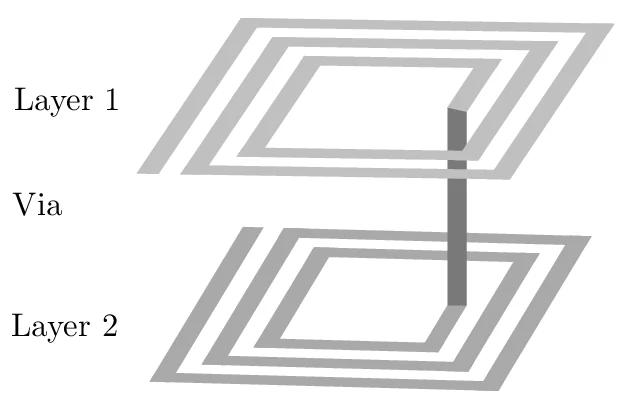
\includegraphics[width=0.4\textwidth]{chapter5_Yassin/images/Stacked-inductor-to-increase-the-inductance-value.png}
    \caption{Stacked inductor structure}
    \label{fig:stacked_inductor}
\end{figure}

%-------------------------------------------------------------
\subsection{Proposed Layout of Choke Inductor}
\label{subsec:choke_layout}

The stacked inductor is designed using the top two metal layers with 7 turns. An inductor shield is placed in an intermediate layer to increase the quality factor without significantly degrading the self-resonance frequency. Narrow inner coils and wider outer coils are used to minimise the impact of the proximity effect.

\begin{figure}[H]
    \centering
    \vspace{-4pt}
    
\includegraphics[width=0.5\textwidth,]{ind.png}
    \caption{Layout of the choke inductor}
    \label{fig:choke_layout}
\end{figure}

%-------------------------------------------------------------
\subsection{Inductance Value of the Choke Inductor}
\label{subsec:inductance_value}

The simulated frequency response of the proposed stacked choke inductor confirms a high nominal inductance value of 20.08\,nH at 1.4\,GHz. the primary self-resonance frequency ($f_\text{SRF1}$) occurs at 3.186\,GHz, followed by higher-order self-resonance points at 10.99\,GHz and 14.55\,GHz. Crucially, having an in-band primary $f_\text{SRF}$ at 3.186\,GHz does not degrade output matching. This is because the parallel resistive feedback network is designed with a sufficiently low resistance value to remain completely dominant over the inductor's high-frequency impedance variations.

\begin{figure}[H]
    \centering
    \vspace{-4pt}
    \includegraphics[width=\textwidth,
    height=8cm]{Lind.png}
    \caption{Inductance value and self-resonance frequency}
    \label{fig:inductance_SRF}
\end{figure}

%-------------------------------------------------------------
\subsection{Quality Factor}
\label{subsec:Q_factor}

\begin{figure}[H]
    \centering
    \vspace{-4pt}
    
\includegraphics[width=0.5\textwidth,height=8cm]{QIND.png}
    \caption{Quality factor of the choke inductor}
    \label{fig:Q_factor}
\end{figure}

%-------------------------------------------------------------
\subsection{Output Impedance from the Choke Inductor and Resistive Feedback}
\label{subsec:output_impedance}
 At low frequencies, the stacked choke's high impedance ($Z_{\text{choke}}$) isolates the active channel from the power rail to preserve forward gain ($S_{21}$). At the 2.8 GHz primary self-resonance, $Z_{\text{choke}}$ peaks at 2.3 k$\Omega$ before rolling off capacitively. Meanwhile, the parallel feedback impedance ($Z_{\text{feedback}}$) remains stable between 200 $\Omega$ and 300 $\Omega$. Because $Z_{\text{feedback}}$ is lower, it dominates the load network as $Z_{\text{choke}}$ drops, masking the inductor's self-resonance and maintaining a stable output match ($S_{22}$).Out-of-band near 10.4 GHz, secondary resonance drops $Z_{\text{choke}}$ to 33.9 $\Omega$ while $Z_{\text{feedback}}$ peaks at 316.8 $\Omega$. This mismatch degrades $S_{22}$ to -6.46 dB and causes an unwanted $S_{21}$ gain recovery to 7.64 dB. To suppress this peaking, a small source-degeneration inductor ($L_s$) is introduced. Its reactance ($j\omega L_s$) is negligible within the 400 MHz to 8 GHz operating band but rises significantly at 10.4 GHz, introducing targeted negative feedback that rolls off out-of-band gain without degrading in-band performance

\begin{figure}[H]
    \centering
    \vspace{-4pt}
    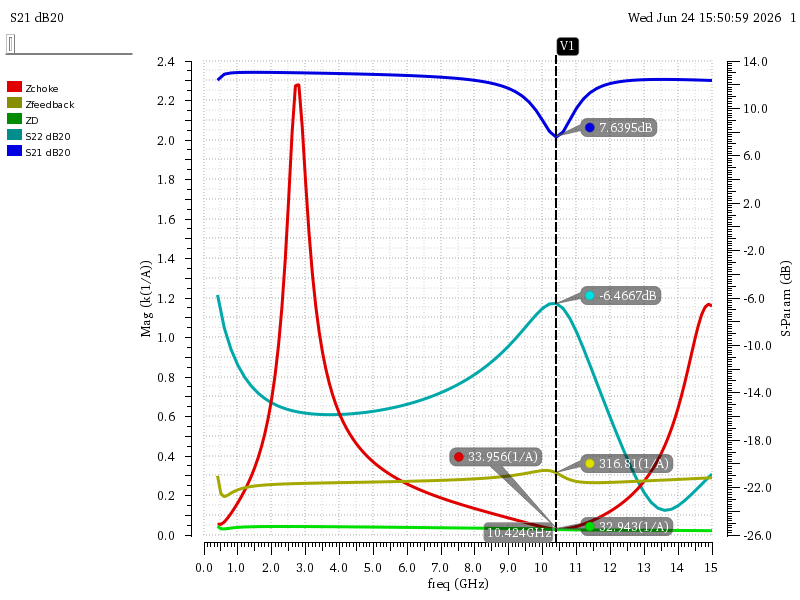
\includegraphics[width=\textwidth,
    height=8cm]{chapter5_Yassin/images/ZCHOKE_ZFDBCK_SP.png}
    \caption{Parallel output impedances of the choke inductor and resistive feedback}
    \label{fig:output_impedances}
\end{figure}

%-------------------------------------------------------------
\subsection{Response After Small Degeneration Inductor}
\label{subsec:degeneration}

Adding a small degeneration inductor reduces the out-of-band gain while introducing no significant change to the in-band performance.
\begin{figure}[H]
    \centering
    \vspace{-4pt}
    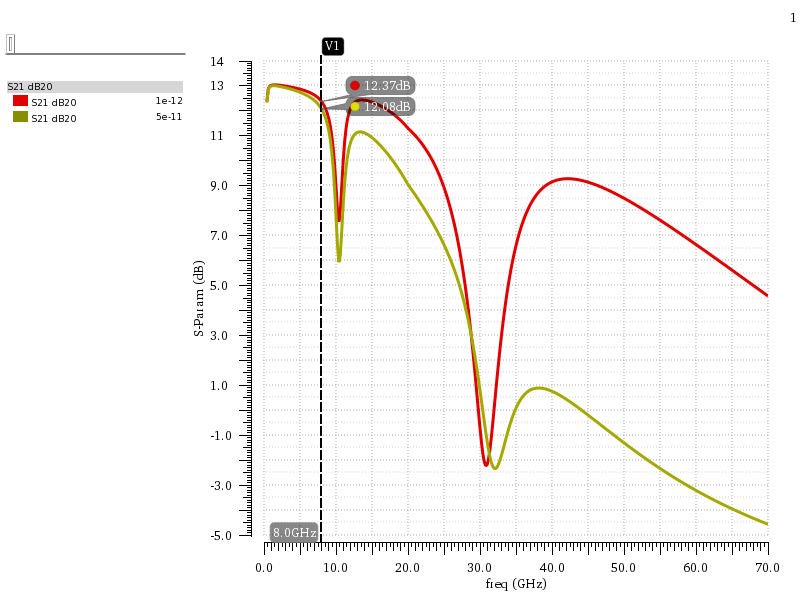
\includegraphics[width=\textwidth,height=8cm]{chapter5_Yassin/images/S21_WITHLdeg.png}
    \caption{S21 with Degeneration inductor }
    \label{fig:degeneration inductor}
\end{figure}
%=============================================================
\section{Proposed Full Layout}
\label{sec:full_layout}

\begin{figure}[H]
    \centering
    \vspace{-4pt}
    
\includegraphics[width=1\textwidth]{finalamp.png}
    \caption{Full layout of the RF amplifier}
    \label{fig:full_layout}
\end{figure}

%=============================================================
\section{Post-Layout Results}
\label{sec:post_layout}

\subsection{Input Matching Across Frequency}
\label{subsec:S11_corners}

\begin{figure}[H]
    \centering
    \vspace{-4pt}
    \includegraphics[width=\textwidth,
    height=8cm]{s11_POST.png}
    \caption{$S_{11}$ across process corners}
    \label{fig:S11_corners}
\end{figure}

%-------------------------------------------------------------
\subsection{Output Matching Across Frequency}
\label{subsec:S22_corners}

\begin{figure}[H]
    \centering
    \vspace{-4pt}
    \includegraphics[width=\textwidth,
    height=8cm]{s22_POST.png}
    \caption{$S_{22}$ across process corners}
    \label{fig:S22_corners}
\end{figure}

%-------------------------------------------------------------
\subsection{Gain Across Frequency}
\label{subsec:S21_corners}

\begin{figure}[H]
    \centering
    \vspace{-4pt}
    \includegraphics[width=\textwidth,
    height=8cm]{s21_POST.png}
    \caption{$S_{21}$ across process corners}
    \label{fig:S21_corners}
\end{figure}

%-------------------------------------------------------------
\subsection{Noise Figure Across Frequency}
\label{subsec:NF_corners}

\begin{figure}[H]
    \centering
    \vspace{-4pt}
    
\includegraphics[width=\textwidth,
    height=8cm]{NF_POST.png}
    \caption{NF across process corners}
    \label{fig:NF_corners}
\end{figure}

%-------------------------------------------------------------
\subsection{OP1dB Across Frequency}
\label{subsec:OP1dB_corners}

\begin{figure}[H]
    \centering
    \vspace{-4pt}
    % Specify both width and a fixed height to force horizontal stretching
    
\includegraphics[width=\textwidth, height=8cm]{OP1DB.png}
    \caption{OP1dB across frequency}
    \label{fig:OP1dB_corners}
\end{figure}

%-------------------------------------------------------------
\subsection{OIP3 Across Frequency}
\label{subsec:OIP3_corners}

The Derivative Superposition technique maintains good linearization across process corners, as the two devices track each other with shifts in $V_{th}$.

\begin{figure}[H]
    \centering
    \vspace{-4pt}
    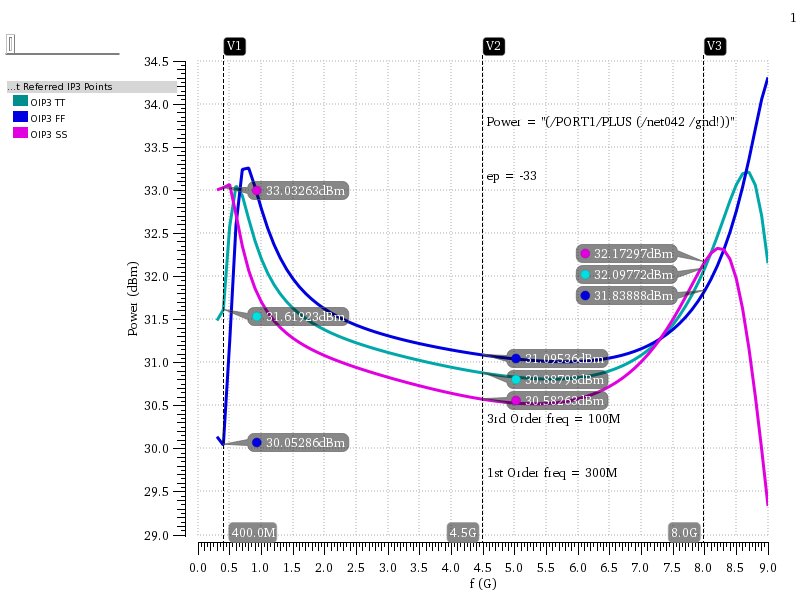
\includegraphics[width=\textwidth,
    height=8cm]{chapter5_Yassin/images/OIP3_POST_pin-3.png}
    \caption{OIP3 across process corners}
    \label{fig:OIP3_corners}
\end{figure}

%-------------------------------------------------------------
\subsection{IIP3 Across Frequency}
\label{subsec:IIP3_corners}

\begin{figure}[H]
    \centering
    \vspace{-4pt}
    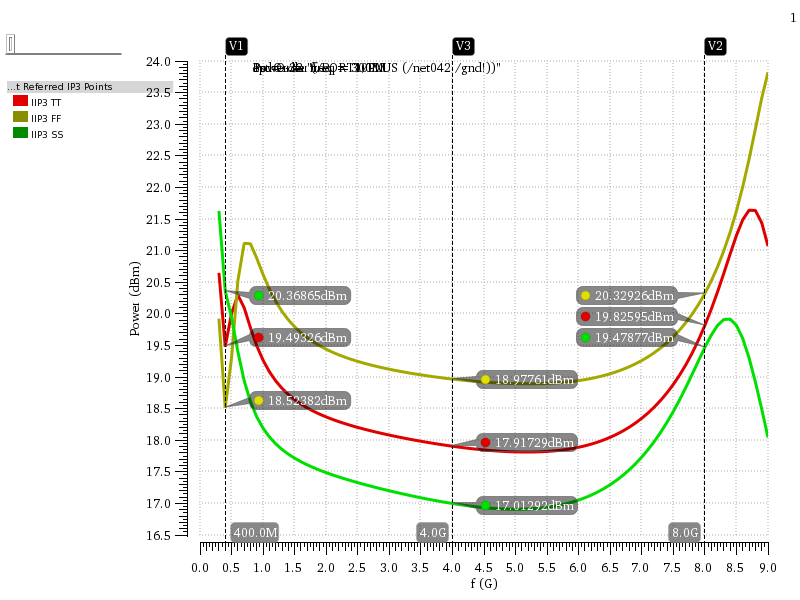
\includegraphics[width=\textwidth,height=8cm]{chapter5_Yassin/images/IIP3_POST_pin-3.png}
    \caption{IIP3 across process corners}
    \label{fig:IIP3_corners}
\end{figure}

%-------------------------------------------------------------
\subsection{OIP3 Across Monte Carlo}
\label{subsec:OIP3_MC}

The Derivative Superposition technique also maintains good linearization across mismatch corners.

\begin{figure}[H]
    \centering
    \vspace{-4pt}
    
\includegraphics[width=\textwidth,height=8cm]{OIP3_MC.png}
    \caption{OIP3 Monte Carlo results}
    \label{fig:OIP3_MC}
\end{figure}

\subsection{KF Across Corners}
\label{subsec:KF_corners}
.
\begin{figure}[H]
    \centering
    \vspace{-4pt}
    
\includegraphics[width=\textwidth,height=8cm]{kf_150G.png}
    \caption{kf across corners}
    \label{fig:kf_corners}
\end{figure}

%-------------------------------------------------------------
\subsection{Out-of-Band Gain}
\label{subsec:out_of_band_gain}

\begin{figure}[H]
    \centering
    \vspace{-4pt}
    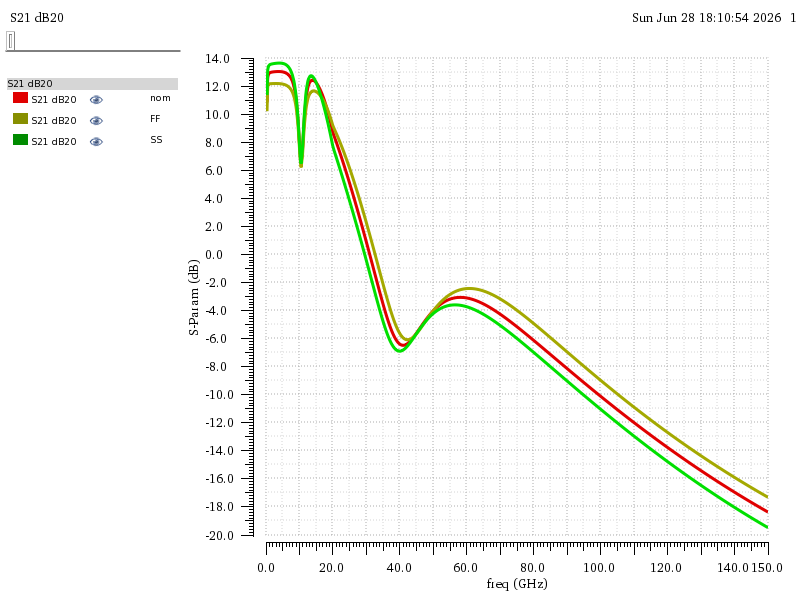
\includegraphics[width=\textwidth,height=8cm]{chapter5_Yassin/images/s21_150G.png}
    \caption{Out-of-band $S_{21}$ across process corners up to 150\,GHz}
    \label{fig:out_of_band_gain}
\end{figure}

%-------------------------------------------------------------
\subsection{DC Power Consumption Across Input Power}
\label{subsec:DC_power}

\begin{figure}[H]
    \centering
    \vspace{-4pt}
    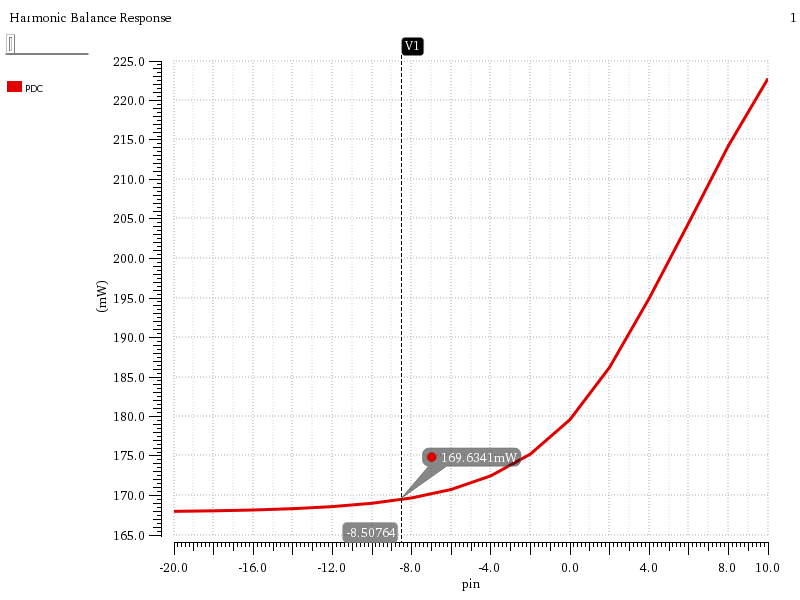
\includegraphics[width=\textwidth,height=8cm]{chapter5_Yassin/images/PDC_PIN.png}
    \caption{DC power consumption vs.\ input power}
    \label{fig:DC_power}
\end{figure}

%-------------------------------------------------------------
\subsection{OIP3 vs.\ Input Power}
\label{subsec:OIP3_vs_pin}

The OIP3 drops by 1\,dB at $P_\text{in} = -8\,\text{dBm}$. Given that the maximum input signal power is $P_\text{in} = -15\,\text{dBm}$, the OIP3 remains constant up to that input power level.
\begin{figure}[H]
    \centering
    \vspace{-4pt}
    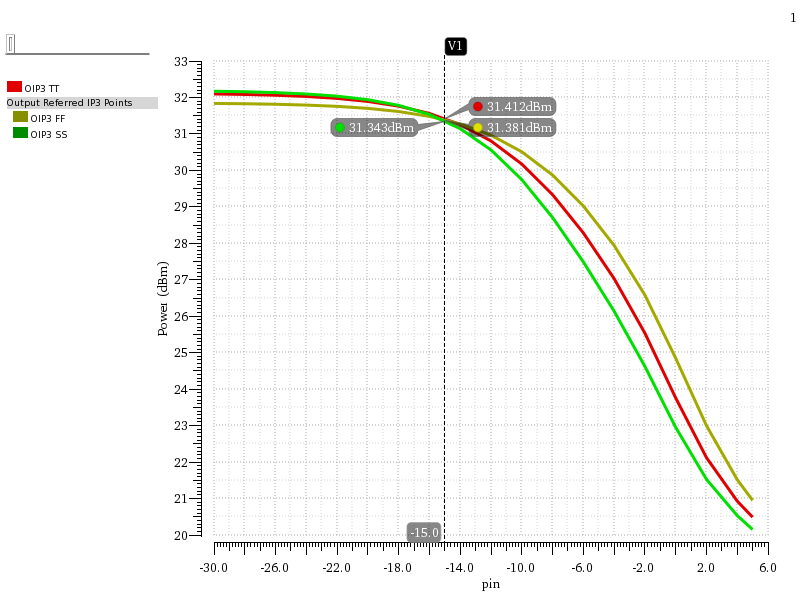
\includegraphics[width=\textwidth,
    height=8cm]{chapter5_Yassin/images/OIP3VSPIN.png}
    \caption{OIP3 VS PIN}
    \label{fig:OIP3 VS PIN}
\end{figure}

%=============================================================
\section{Post-Layout Integration Results of RF Amplifier with DSA}
\label{sec:post_layout_integration}

This integration was performed on the post-layout of both the RF amplifier and the DSA. Since the output matching of the DSA and the input matching of the RF amplifier are well matched across the wideband, the integration yields nearly identical results to the individual post-layout simulations.

%-------------------------------------------------------------
\subsection{$S_{11}$ Across Frequency}
\label{subsec:int_S11}

\begin{figure}[H]
    \centering
    \vspace{-4pt}
    
\includegraphics[width=0.75\textwidth]{S11_TT.png}
    \caption{$S_{11}$ across frequency}
    \label{fig:int_S11}
\end{figure}

%-------------------------------------------------------------
\subsection{$S_{22}$ Across Frequency}
\label{subsec:int_S22}

\begin{figure}[H]
    \centering
    \vspace{-4pt}
    
\includegraphics[width=0.75\textwidth]{S22_TT.png}
    \caption{$S_{22}$ across frequency}
    \label{fig:int_S22}
\end{figure}

%-------------------------------------------------------------
\subsection{Attenuation States Across Frequency}
\label{subsec:int_atten_states}

\begin{figure}[H]
    \centering
    \vspace{-4pt}
    
\includegraphics[width=0.75\textwidth]{S21_TT.png}
    \caption{Attenuation states across frequency}
    \label{fig:int_atten_states}
\end{figure}

%-------------------------------------------------------------
\subsection{DNL Across States for Different Frequencies}
\label{subsec:int_DNL}

\begin{figure}[H]
    \centering
    \vspace{-4pt}
    
\includegraphics[width=0.75\textwidth]{DNL_TT.png}
    \caption{DNL across states for different frequencies}
    \label{fig:int_DNL}
\end{figure}

%-------------------------------------------------------------
\subsection{IIP3 and OIP3 Across States}
\label{subsec:int_IIP3_OIP3}

The results demonstrate the successful Attenuator--Amplifier topology, which keeps OIP3 constant while IIP3 increases by 1\,dB per attenuation state.

\begin{figure}[H]
    \centering
    \vspace{-4pt}
    
\includegraphics[width=0.75\textwidth]{OIP3_STATES.png}
    \caption{OIP3 across attenuation states}
    \label{fig:int_OIP3_states}
\end{figure}

%-------------------------------------------------------------
\subsection{Noise Figure Across Frequency}
\label{subsec:int_NF}

\begin{figure}[H]
    \centering
    \vspace{-4pt}
    
\includegraphics[width=0.75\textwidth]{NF_TT.png}
    \caption{NF across frequency}
    \label{fig:int_NF}
\end{figure}

%-------------------------------------------------------------
\subsection{Attenuation States Across FF Corner}
\label{subsec:int_atten_FF}

\begin{figure}[H]
    \centering
    \vspace{-4pt}
    
\includegraphics[width=0.75\textwidth]{S21_FF.png}
    \caption{Attenuation states across FF corner}
    \label{fig:int_atten_FF}
\end{figure}

%-------------------------------------------------------------
\subsection{DNL Across FF Corner}
\label{subsec:int_DNL_FF}

\begin{figure}[H]
    \centering
    \vspace{-4pt}
    
\includegraphics[width=0.75\textwidth]{DNL_FF.png}
    \caption{DNL across FF corner}
    \label{fig:int_DNL_FF}
\end{figure}

%-------------------------------------------------------------
\subsection{Attenuation States Across SS Corner}
\label{subsec:int_atten_SS}

\begin{figure}[H]
    \centering
    \vspace{-4pt}
    
\includegraphics[width=0.75\textwidth]{S21_SS.png}
    \caption{Attenuation states across SS corner}
    \label{fig:int_atten_SS}
\end{figure}

%-------------------------------------------------------------
\subsection{DNL Across SS Corner}
\label{subsec:int_DNL_SS}

\begin{figure}[H]
    \centering
    \vspace{-4pt}
    
\includegraphics[width=0.75\textwidth]{DNL_SS.png}
    \caption{DNL across SS corner}
    \label{fig:int_DNL_SS}
\end{figure}
%\renewcommand{\bibname}{References}
%\bibliographystyle{ieeetr}
%\bibliography{chapter5_Yassin/refs}
